\section{Outputs}
  In this penultimate section, I will share some of the outputs the project has delivered. I will use these to reflect on the different parts of the project
  each output is associated with. To do this reflection I will use the Experience, Reflect, Action (ESA) framework founded by Melanie Jasper (2003, p.2).

  \begin{figure}[H]
    \centering
    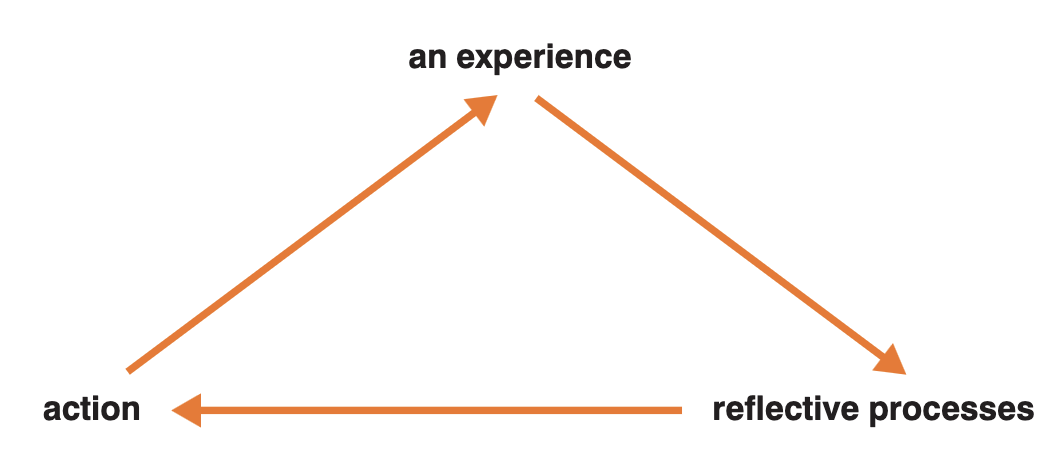
\includegraphics[width=8cm]{assets/eraReflection.png}
    \caption{ERA reflection model founded by Jasper (2003, p.2).}
    \label{fig:eraReflection}
  \end{figure}  

  \subsection{Burn-up Charts}
  \label{sec:burnup}

  \textbf{Experience} -

  \textbf{Reflection} -

  \textbf{Action} -

  \begin{figure}[H]
    \centering
    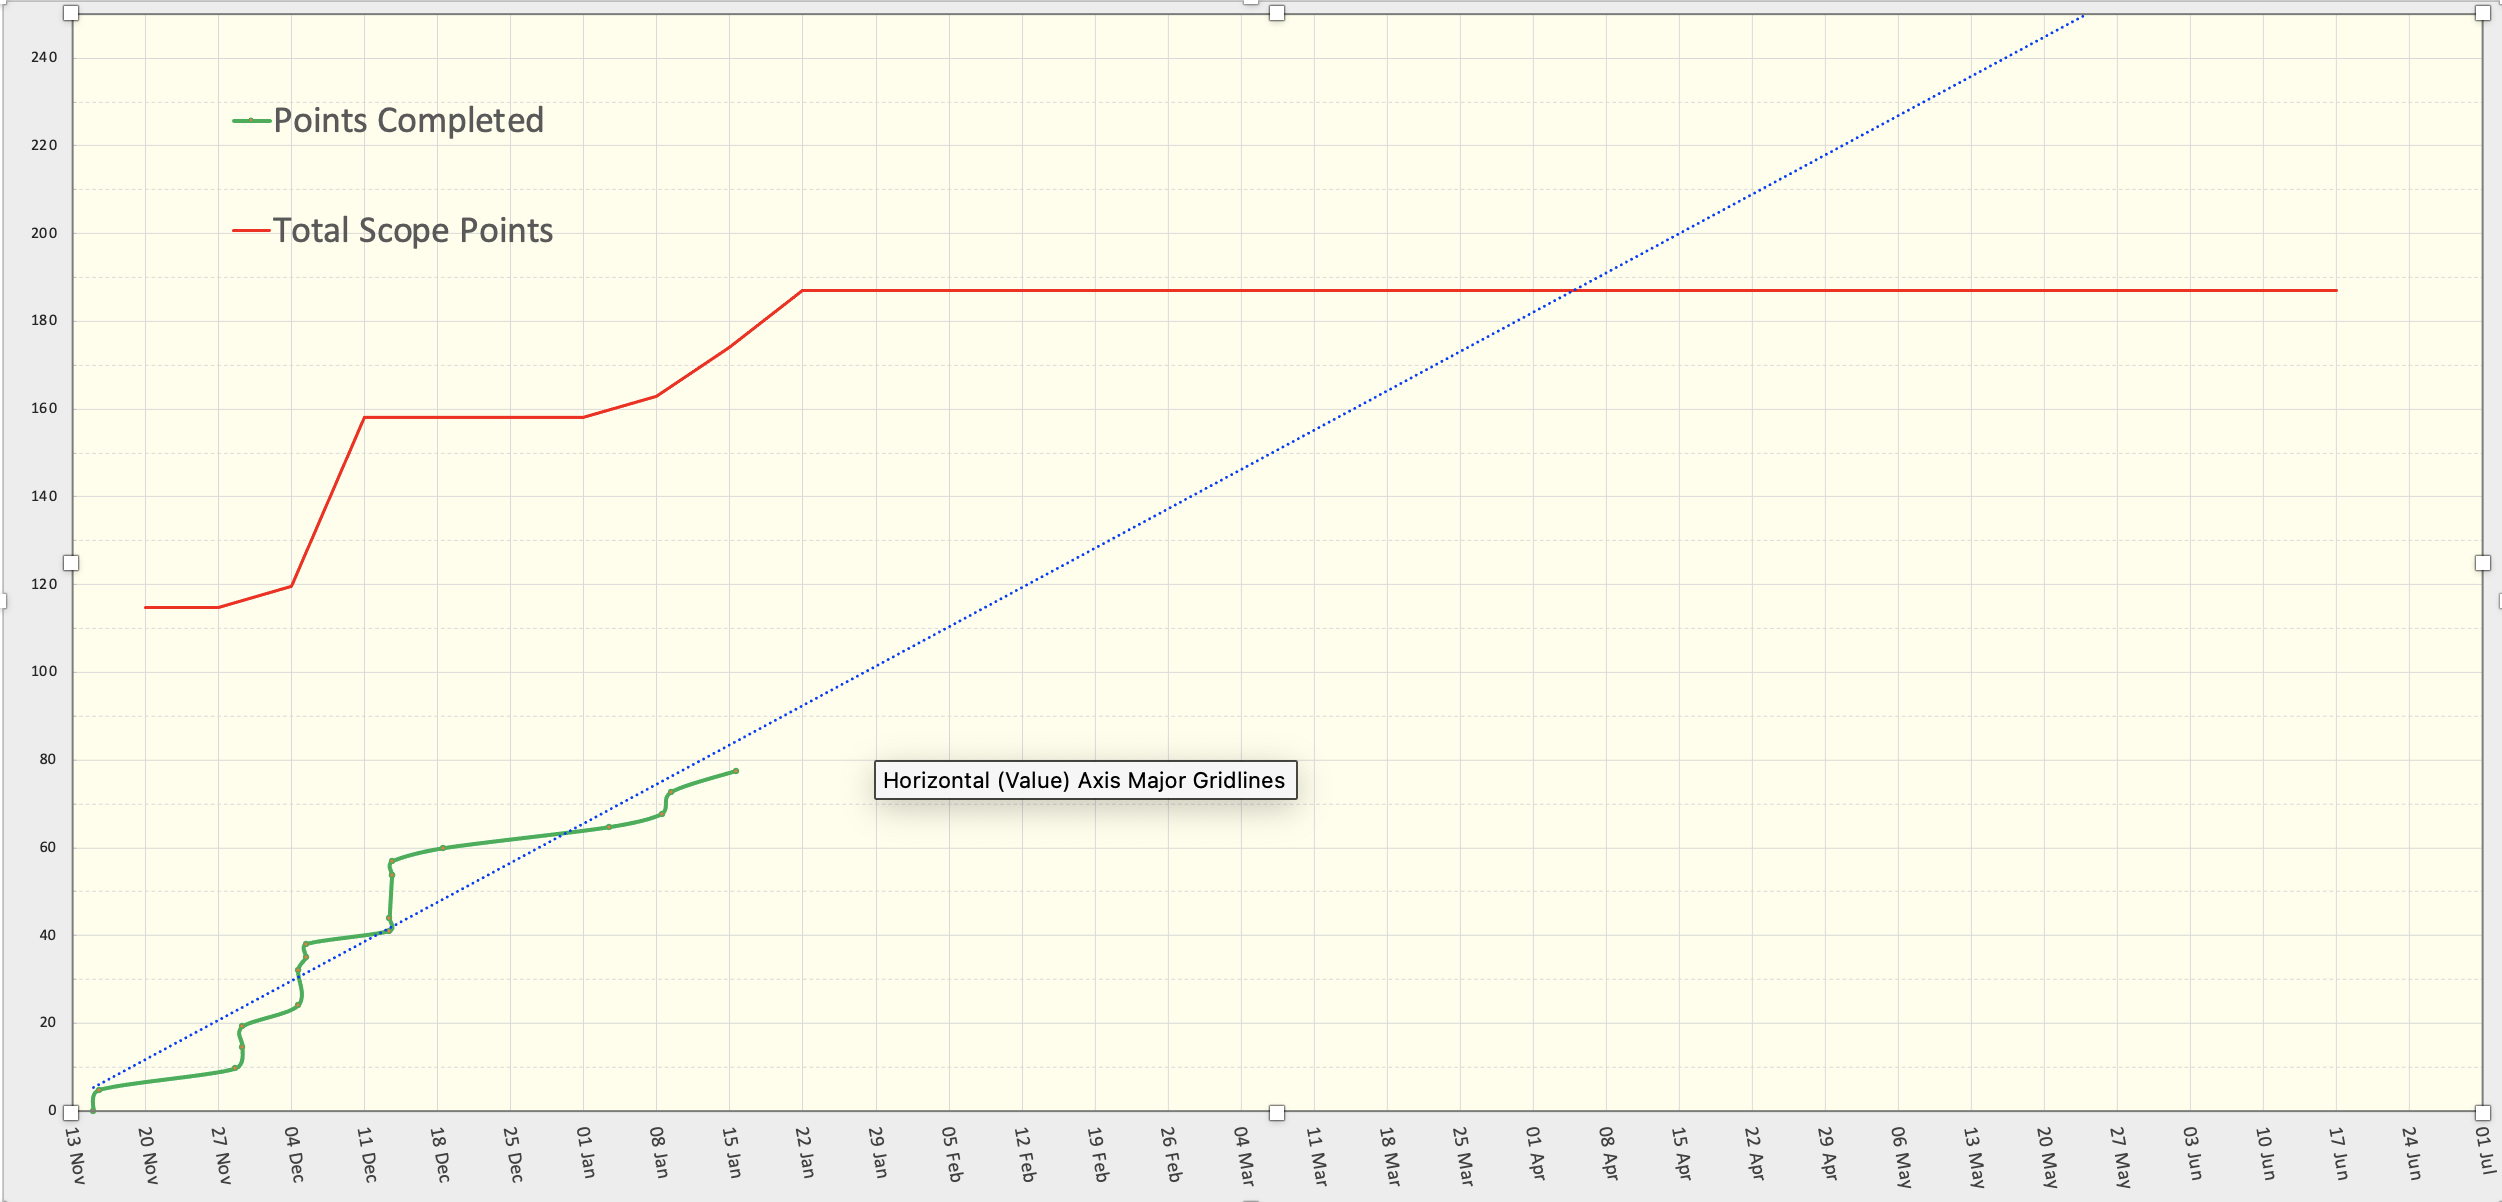
\includegraphics[width=6cm]{assets/outputs/burnups/01-16.png}
    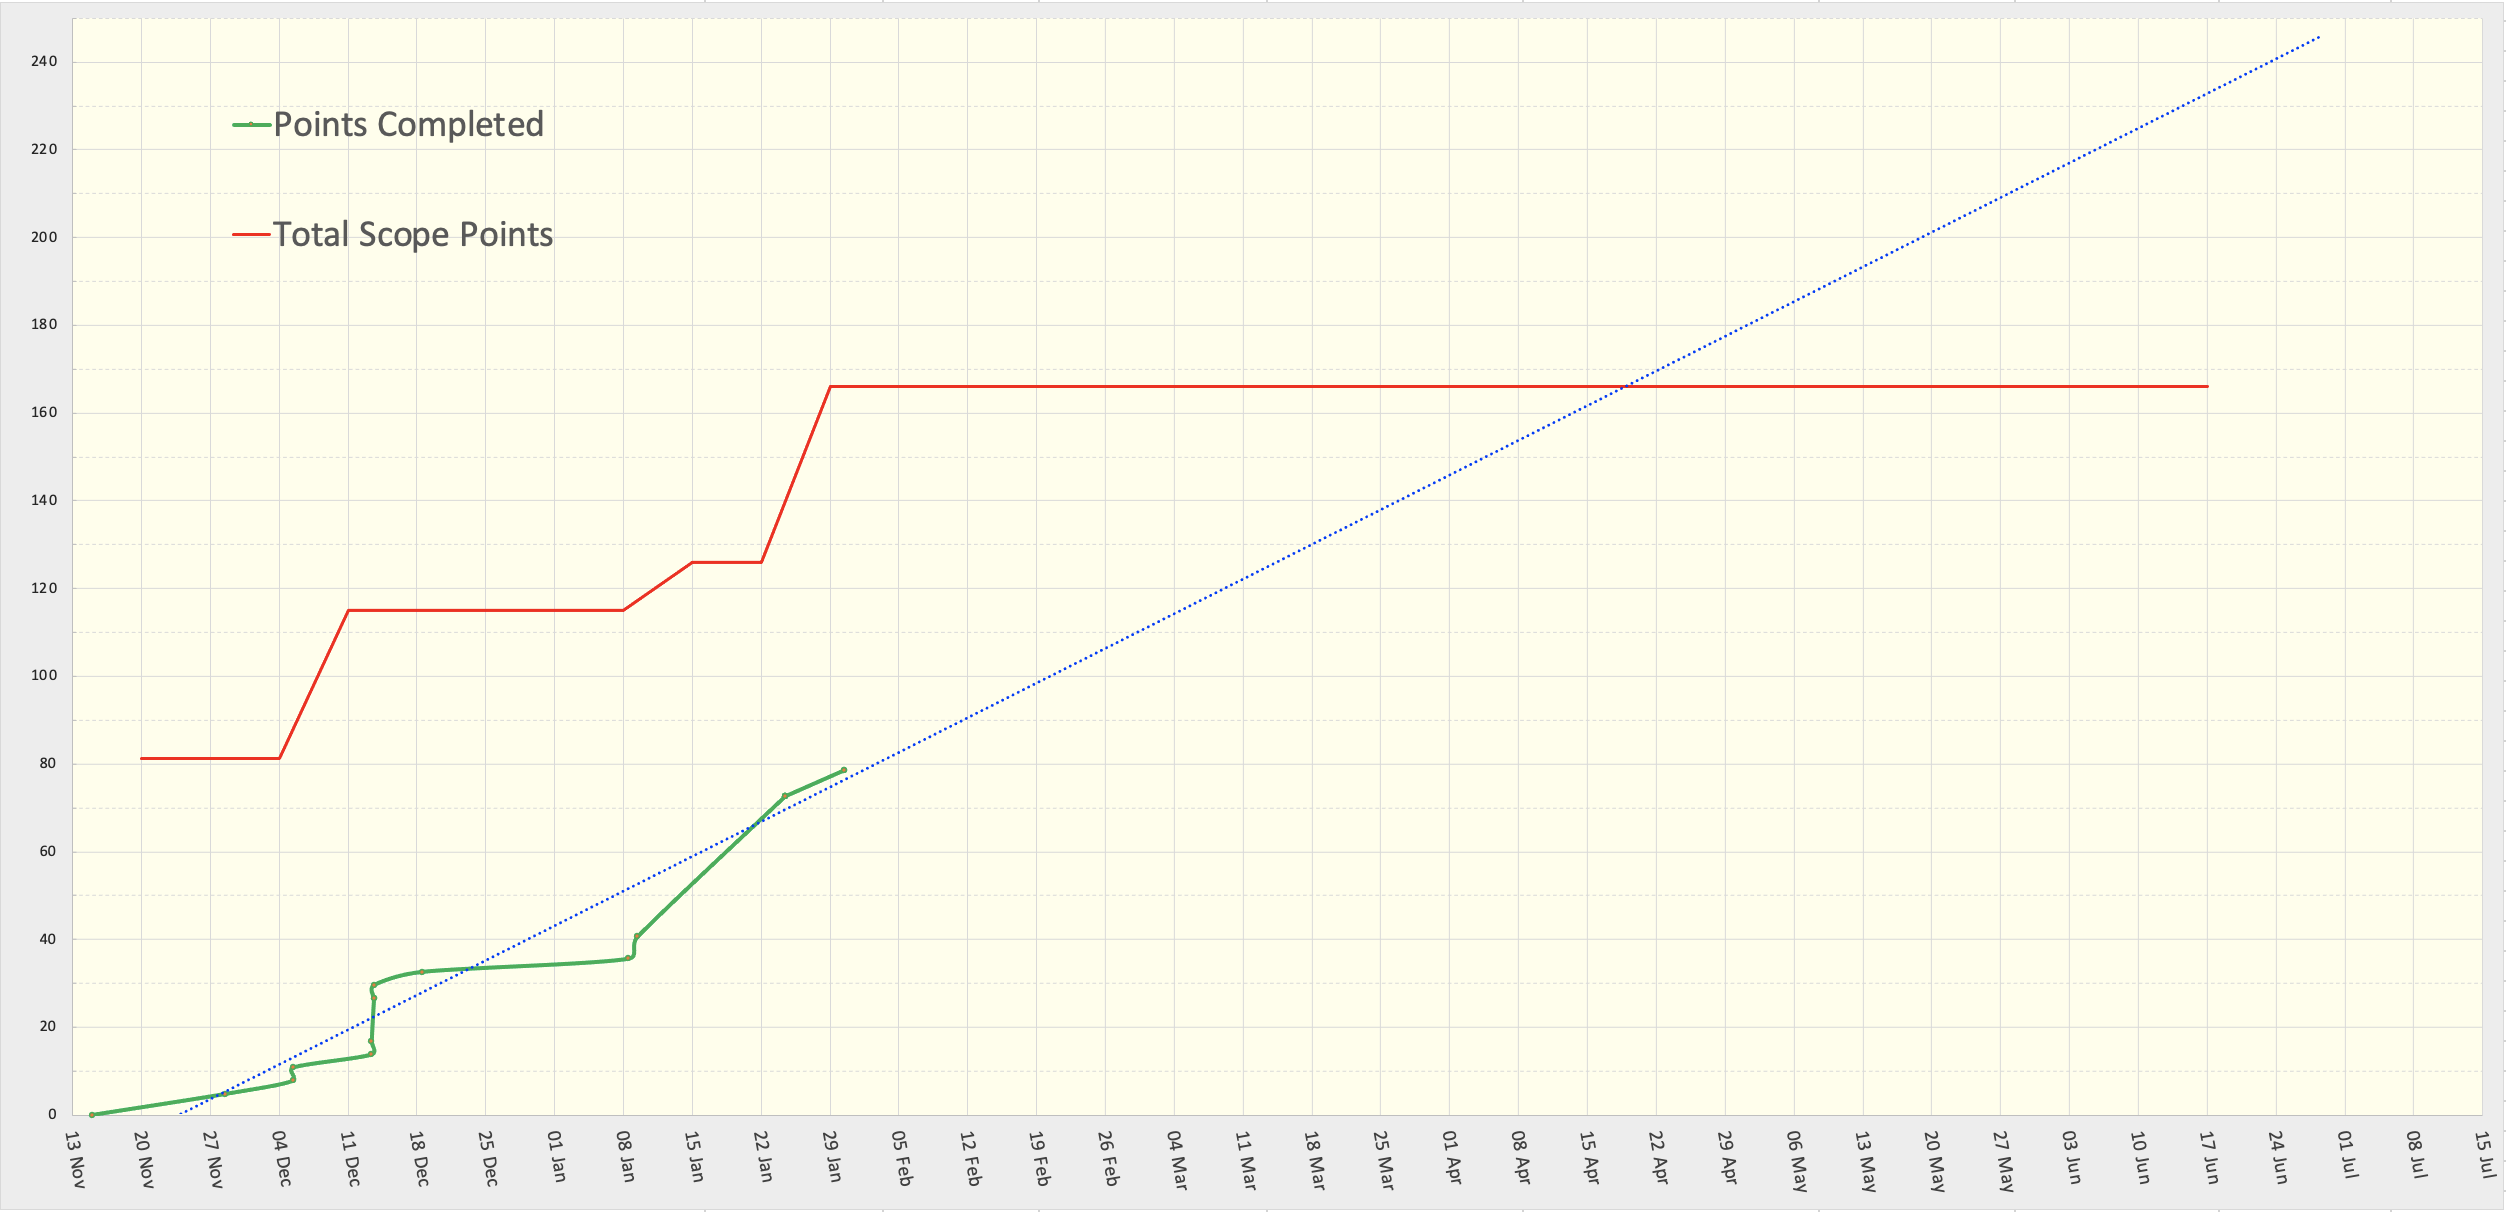
\includegraphics[width=6cm]{assets/outputs/burnups/01-30.png}
    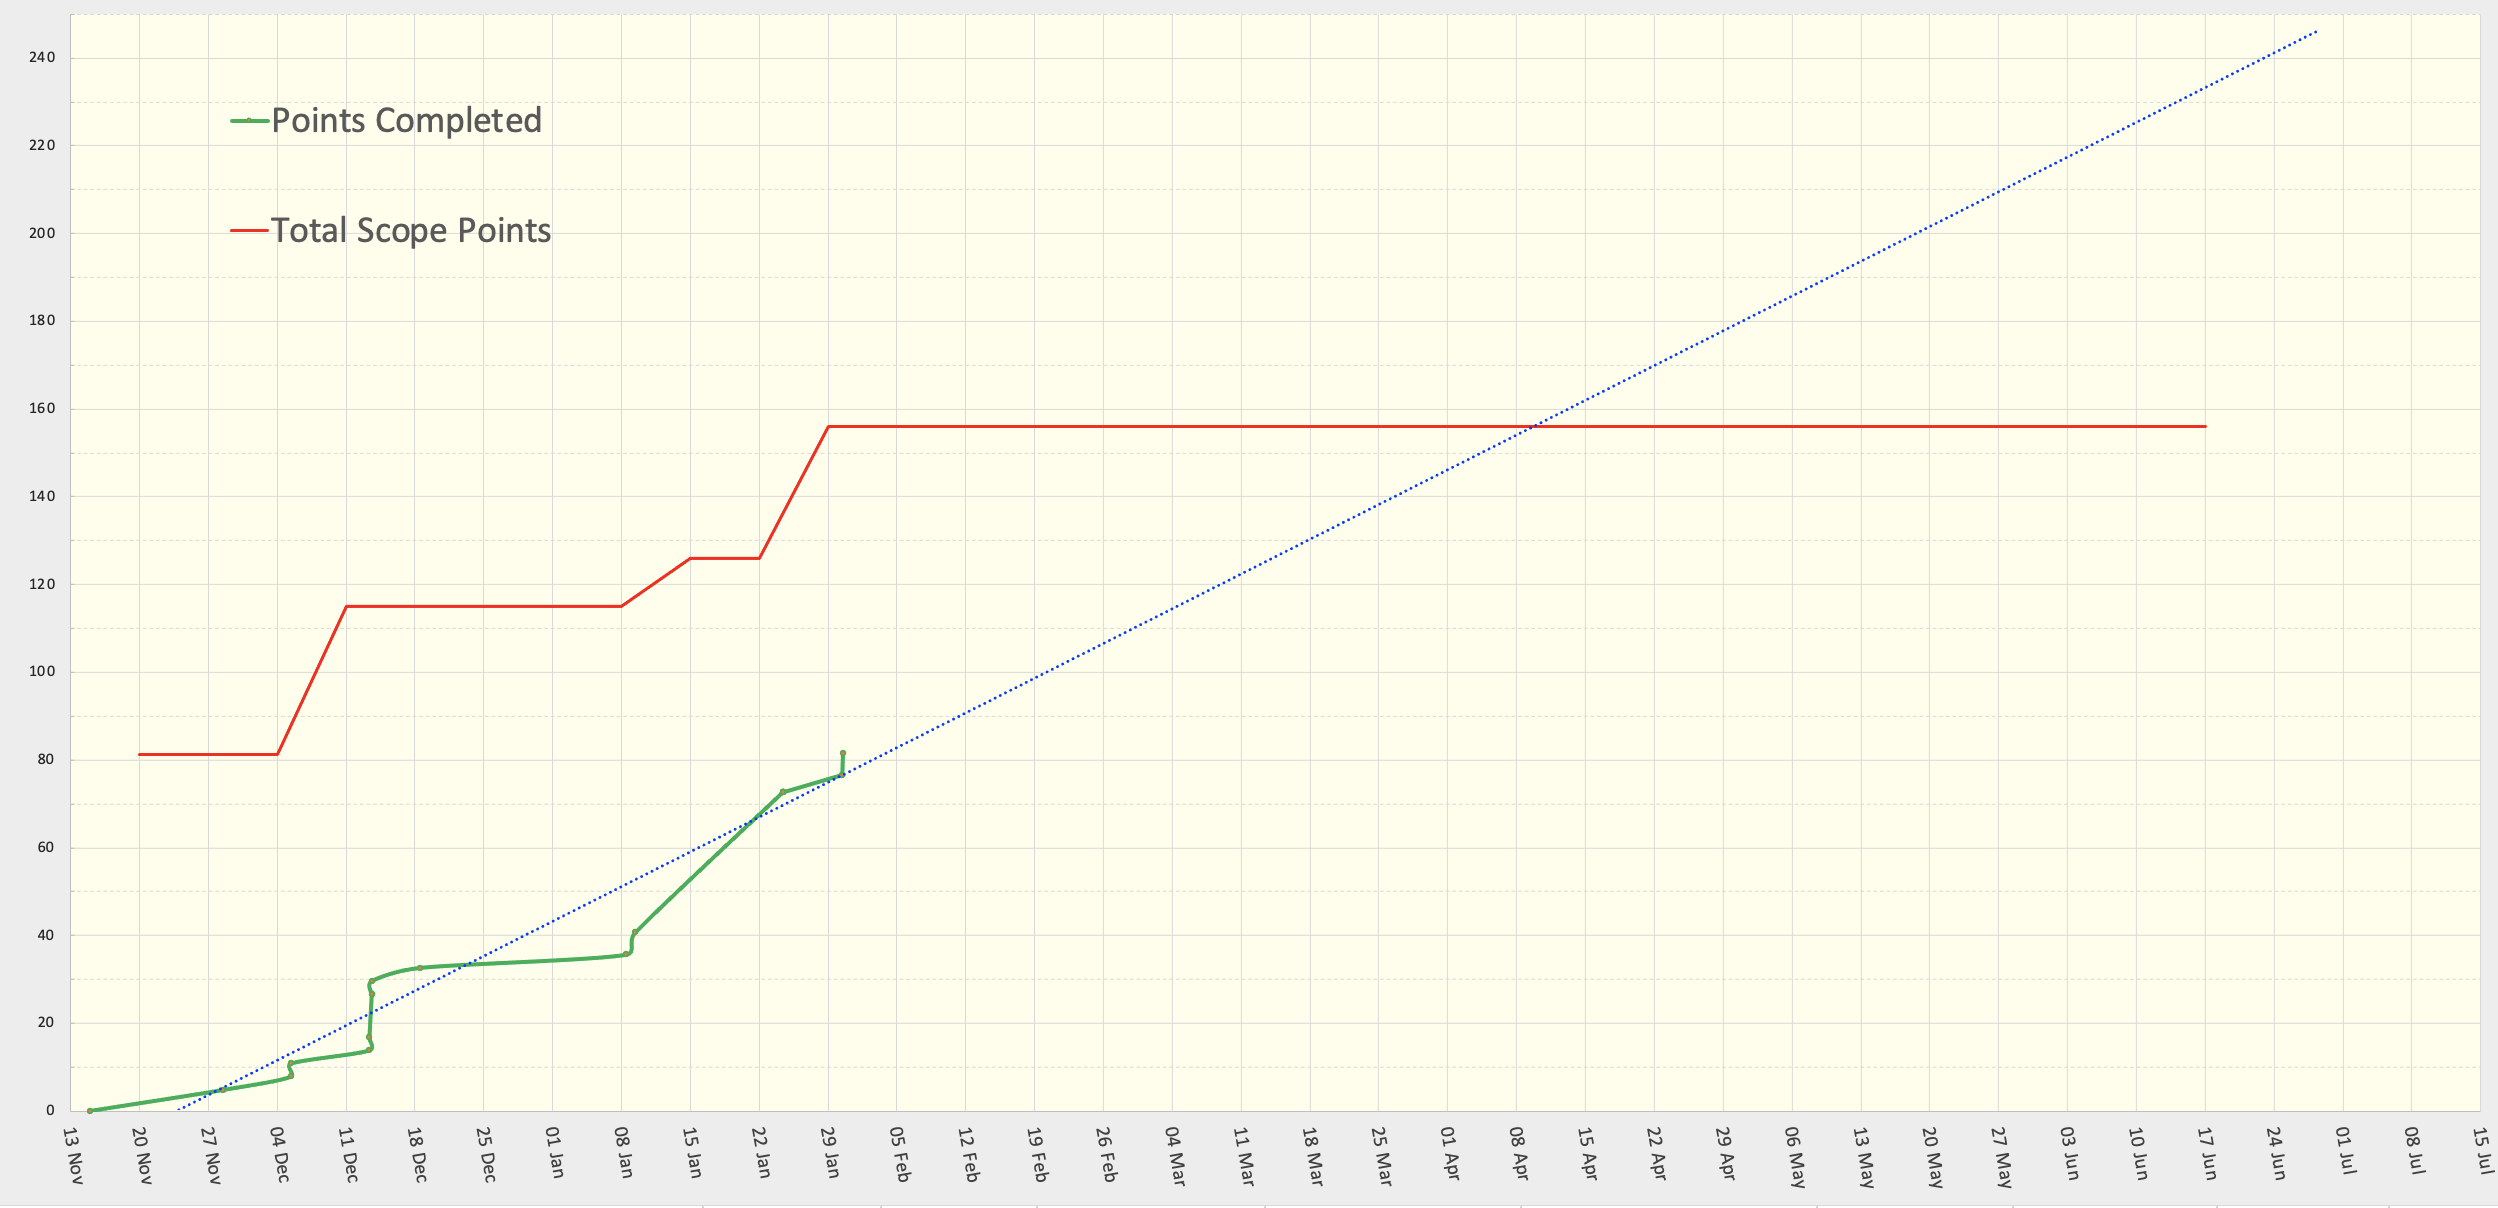
\includegraphics[width=6cm]{assets/outputs/burnups/02-05.png}
    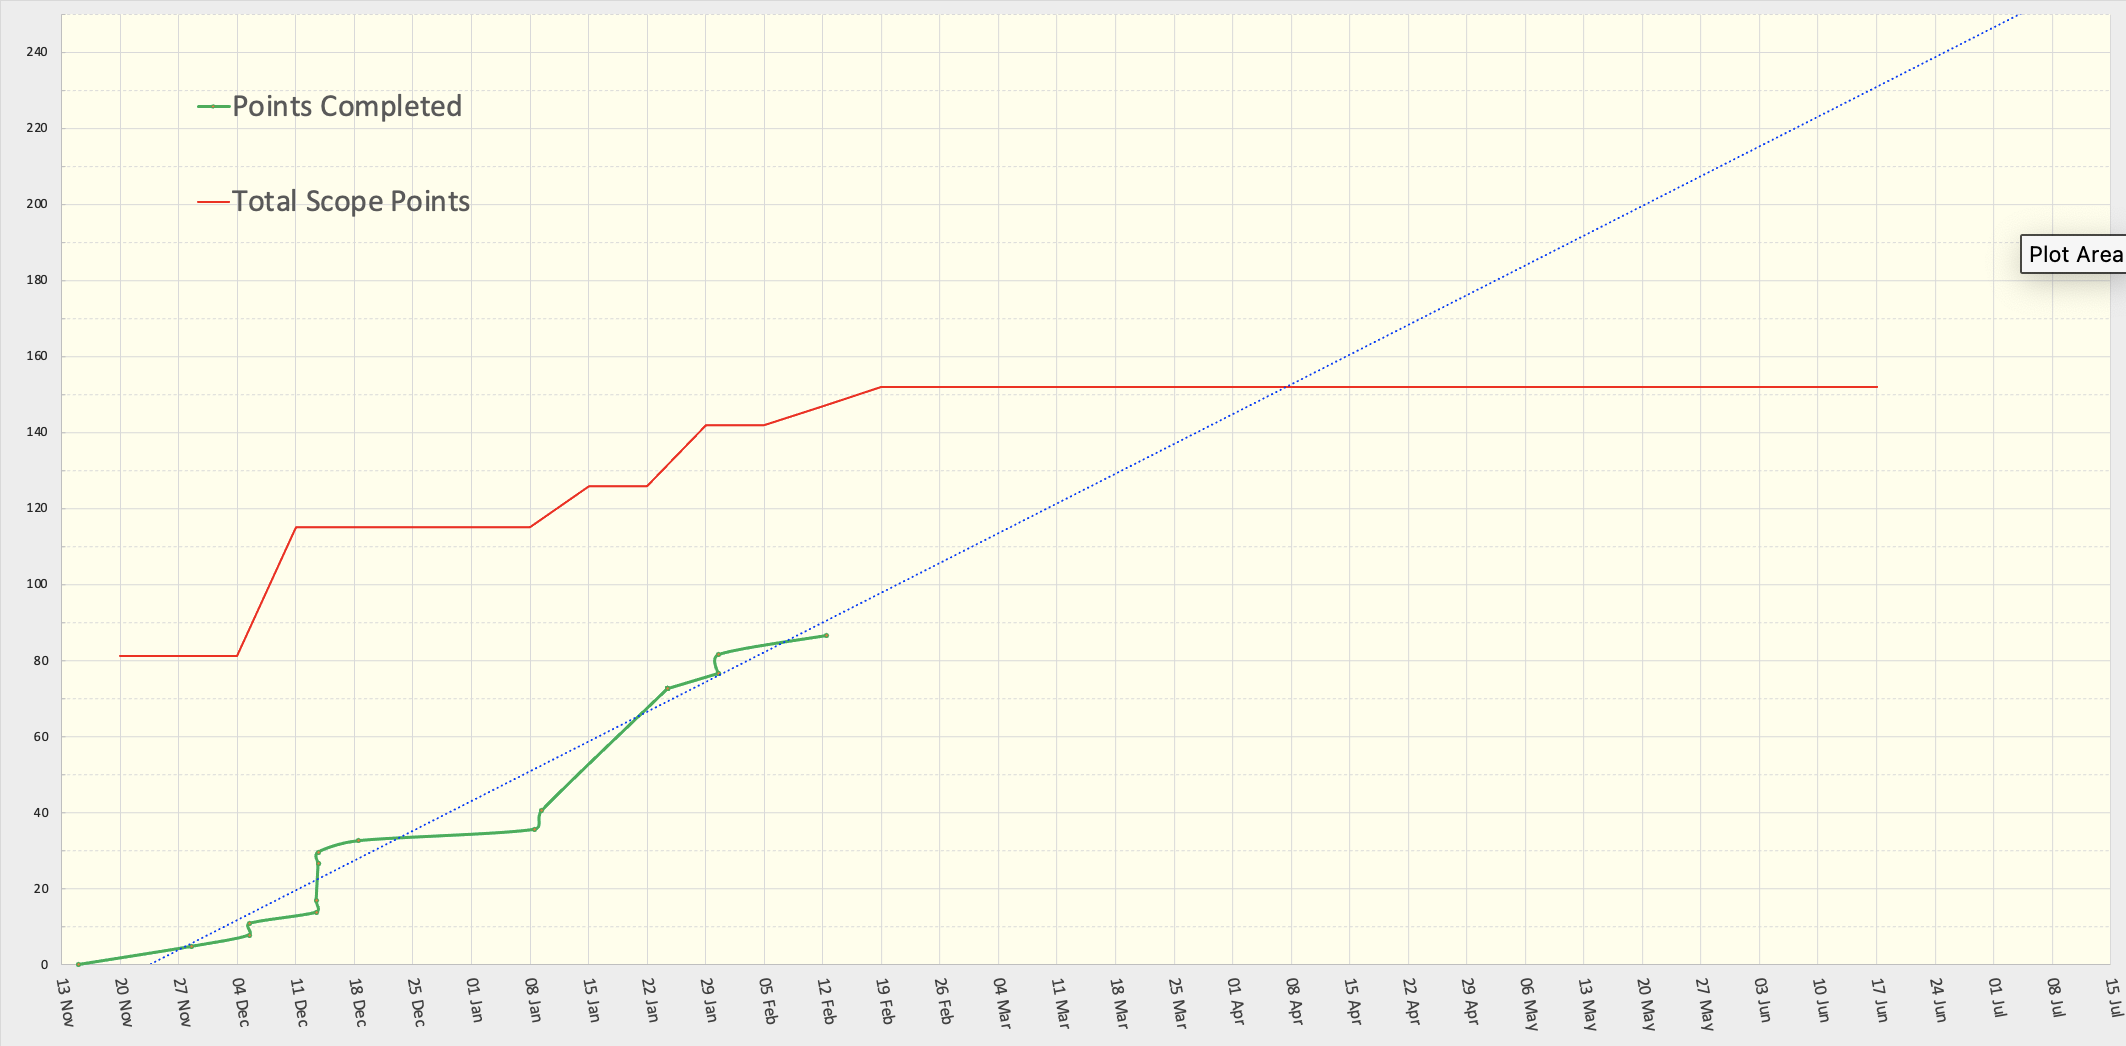
\includegraphics[width=6cm]{assets/outputs/burnups/02-14.png}
    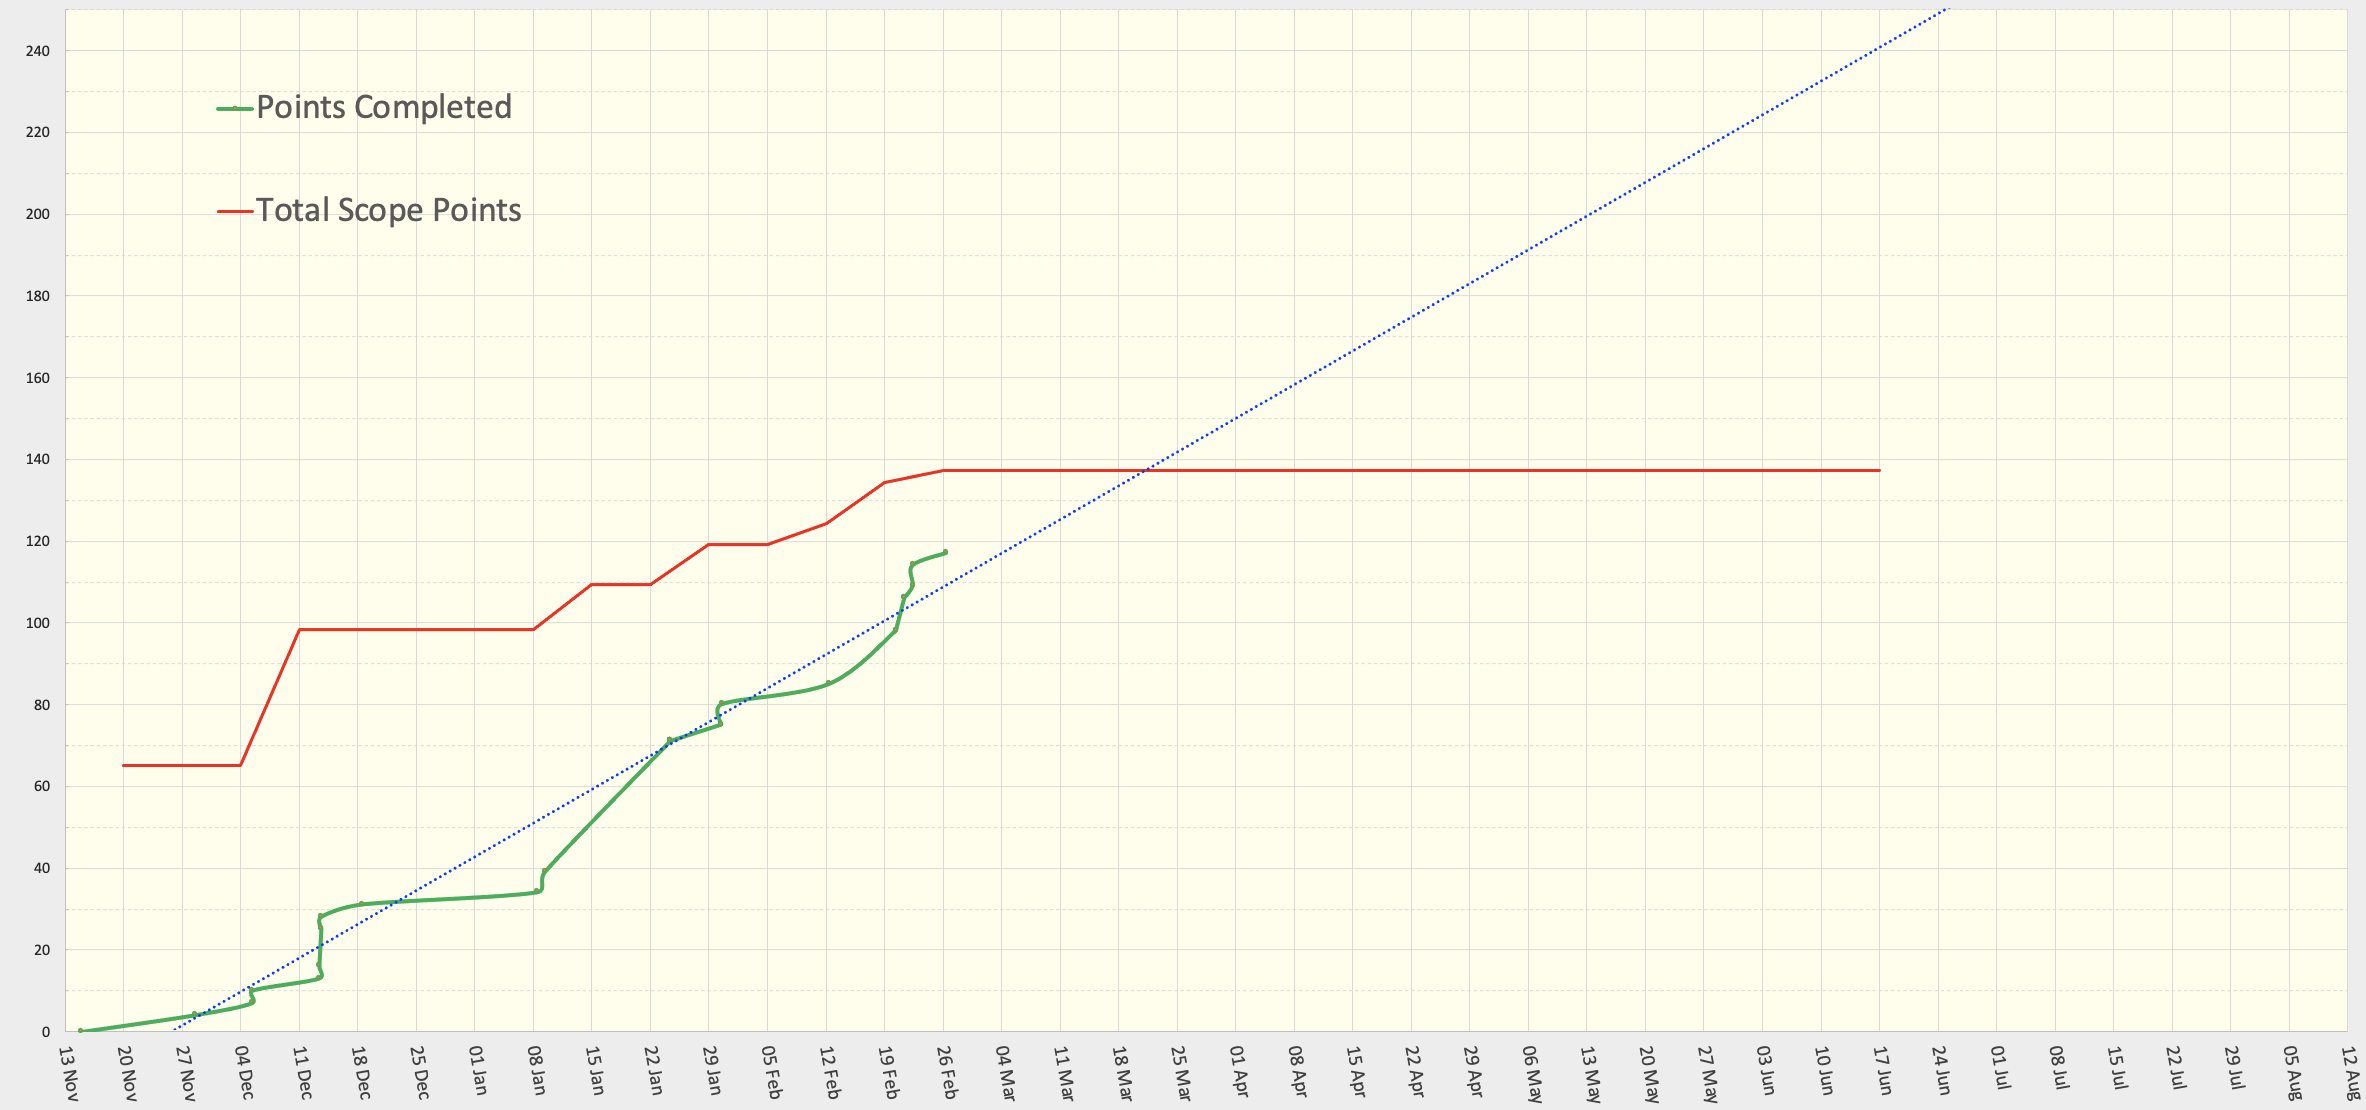
\includegraphics[width=6cm]{assets/outputs/burnups/02-27.png}
    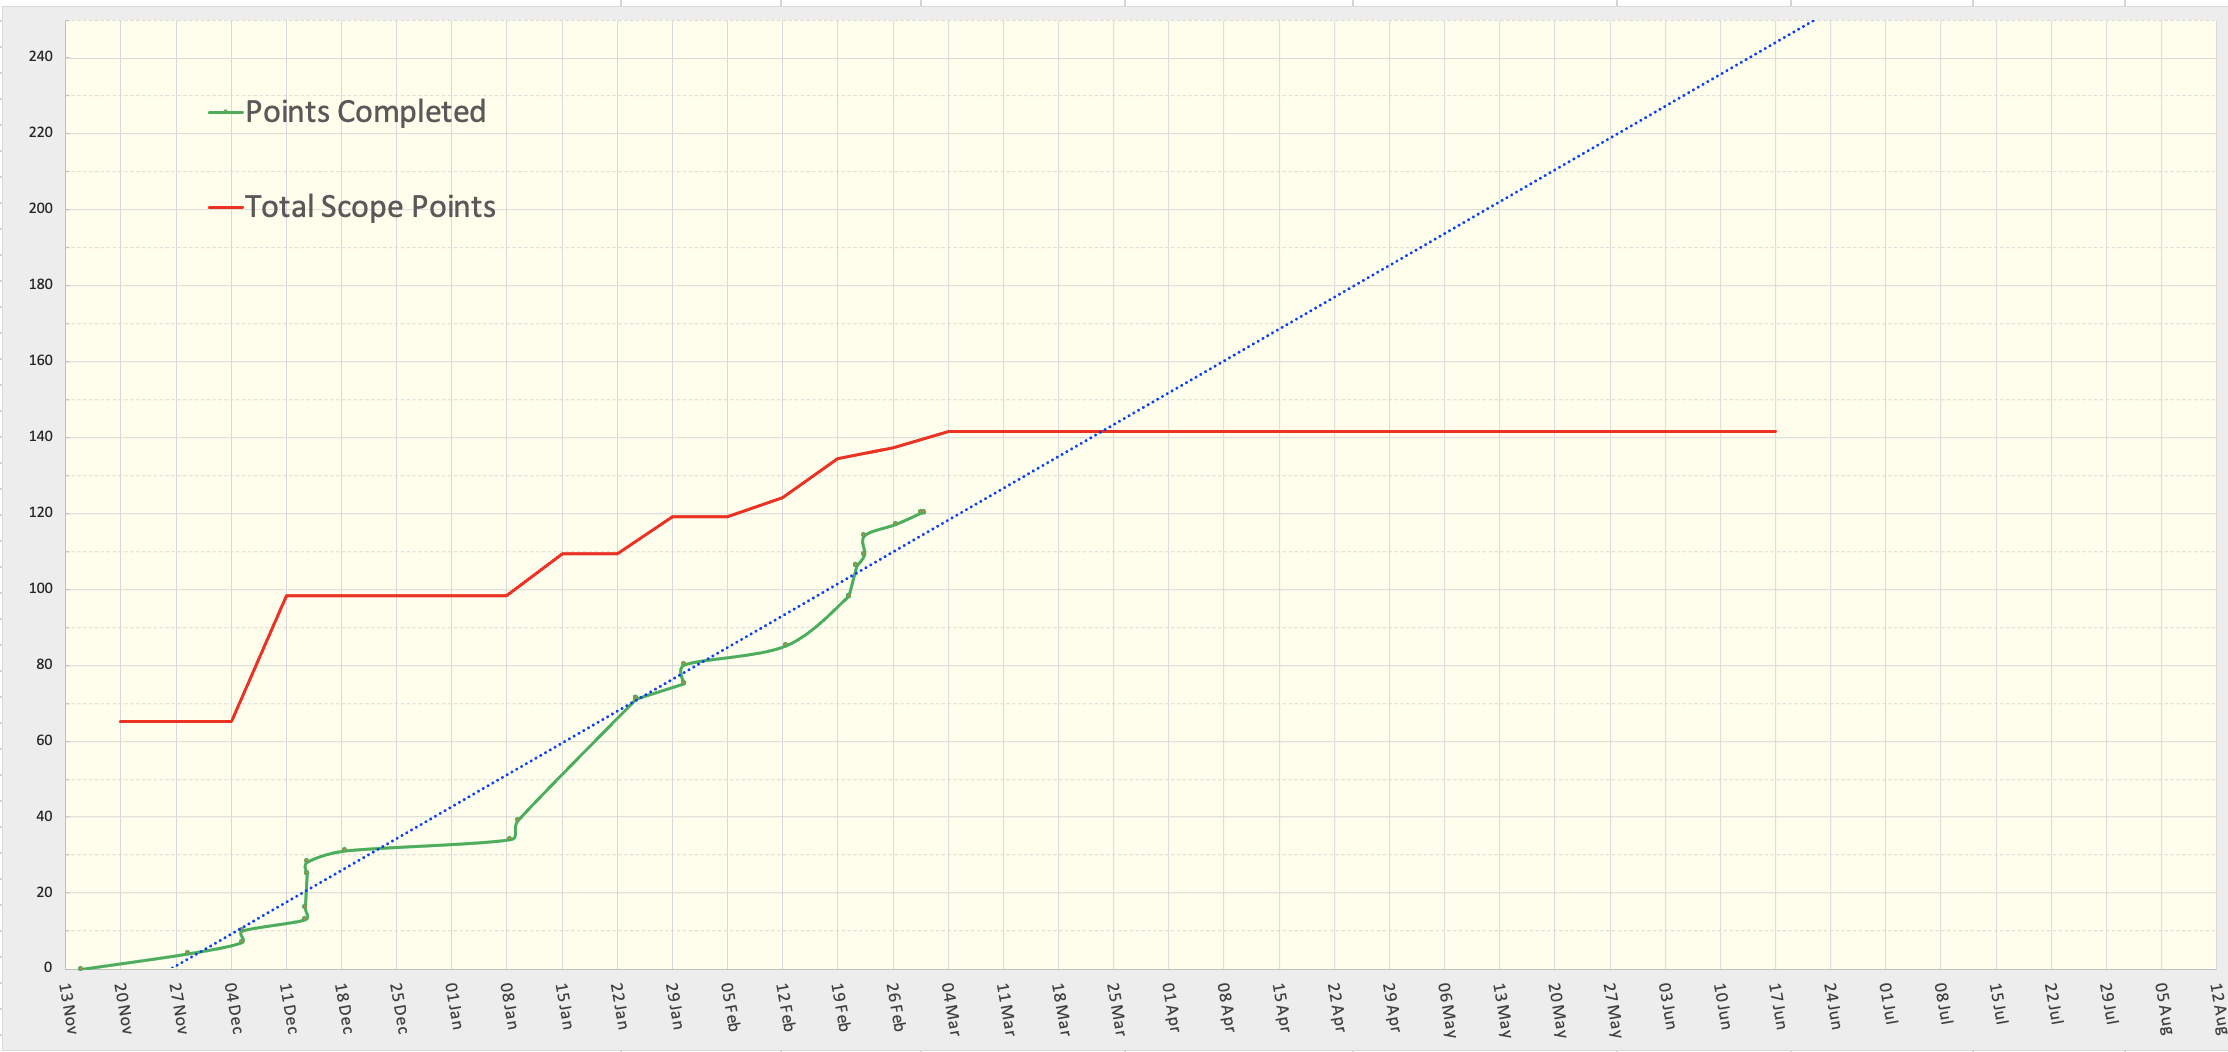
\includegraphics[width=6cm]{assets/outputs/burnups/03-03.png}
    \caption{Burn-up charts throughout the project.}
    \label{fig:burnups}
  \end{figure}

  \newpage
  \subsection{Final System Architecture}

  \textbf{Experience} - A diagram of the final architecture has been created to help both current and new team members understand how the system works.
  It's important to note that the old static lambda and associated schedule events and keyspaces will be removed over time as confidence in the new system 
  grows. This diagram will be used in our internal documentation, such as technical designs and threat models.

  \vspace{0.2cm}
  \textbf{Reflection} - For this project we had an initial design that was created during the spike, which consisted of a publish/subscribe model using
  AWS SNS and SQS (Amazon Web Services, 2024b and 2023c). Other than a separate queue to handle internal re-queuing of events and a garbage collector to 
  extract and simplify some logic, the main architecture didn't change. I think this was a mistake. There were two keys issues the spike found with the design,
  these being complexity of copying over data from the catalogue redis to the schedule redis and an inability to parallelise notifications. A solution to this 
  was offered and in the \hyperref[sec:dynamo]{\textbf{next section}} of this report I will discuss it. 

  The reasons for not going down this alternate approach was in part due to the spike taking longer than expected. Due to this there was no priority placed 
  on further discovery of this alternative solution, as we wanted to start the work straight away. The copying over of data hurt development time due to 
  it's complexity and caused countless bugs and errors that could have been avoided. 
  
  Part way through the project the development team realised that a mistake had been made but had to continue with the original solution. 
  Speaking for myself, this lowered my morale and I found it very frustrating that time was not given to the alternate solution we had suggested during 
  the spike.

  Despite all this it's extremely important to note that the system works exactly as intended and meets all the criteria that was expected. Schedules are 
  now much more up to date and thanks to comparison tests we are able to see that the output is correct.

  \vspace{0.2cm}
  \textbf{Action} - Time was not on our side for this project. There was a lot of pressure to start this project as soon as possible to finish off the 
  schedule pipeline work and have it ready for partners to use.

  Scope creep (Martins, 2023) and lack of time-boxing for the spike ate away at this time and meant later findings in the spike were not explored and we 
  instead opted for the architecture that was similar to the catalogue pipeline. In the future spikes should be time-boxed to stop this creep, 
  so we can review findings earlier and explore a different direction if one has been identified.

  The alternate design also used new AWS services we hadn't used before, more time was needed to research this and understand it. Better spike planning 
  would help, but more general training around AWS services and how to implement them could be encouraged through official training or through side-project
  time (Robinson, 2018), which is something the BBC does offer.

  \begin{landscape}
    \begin{figure}[H]
      \centering
      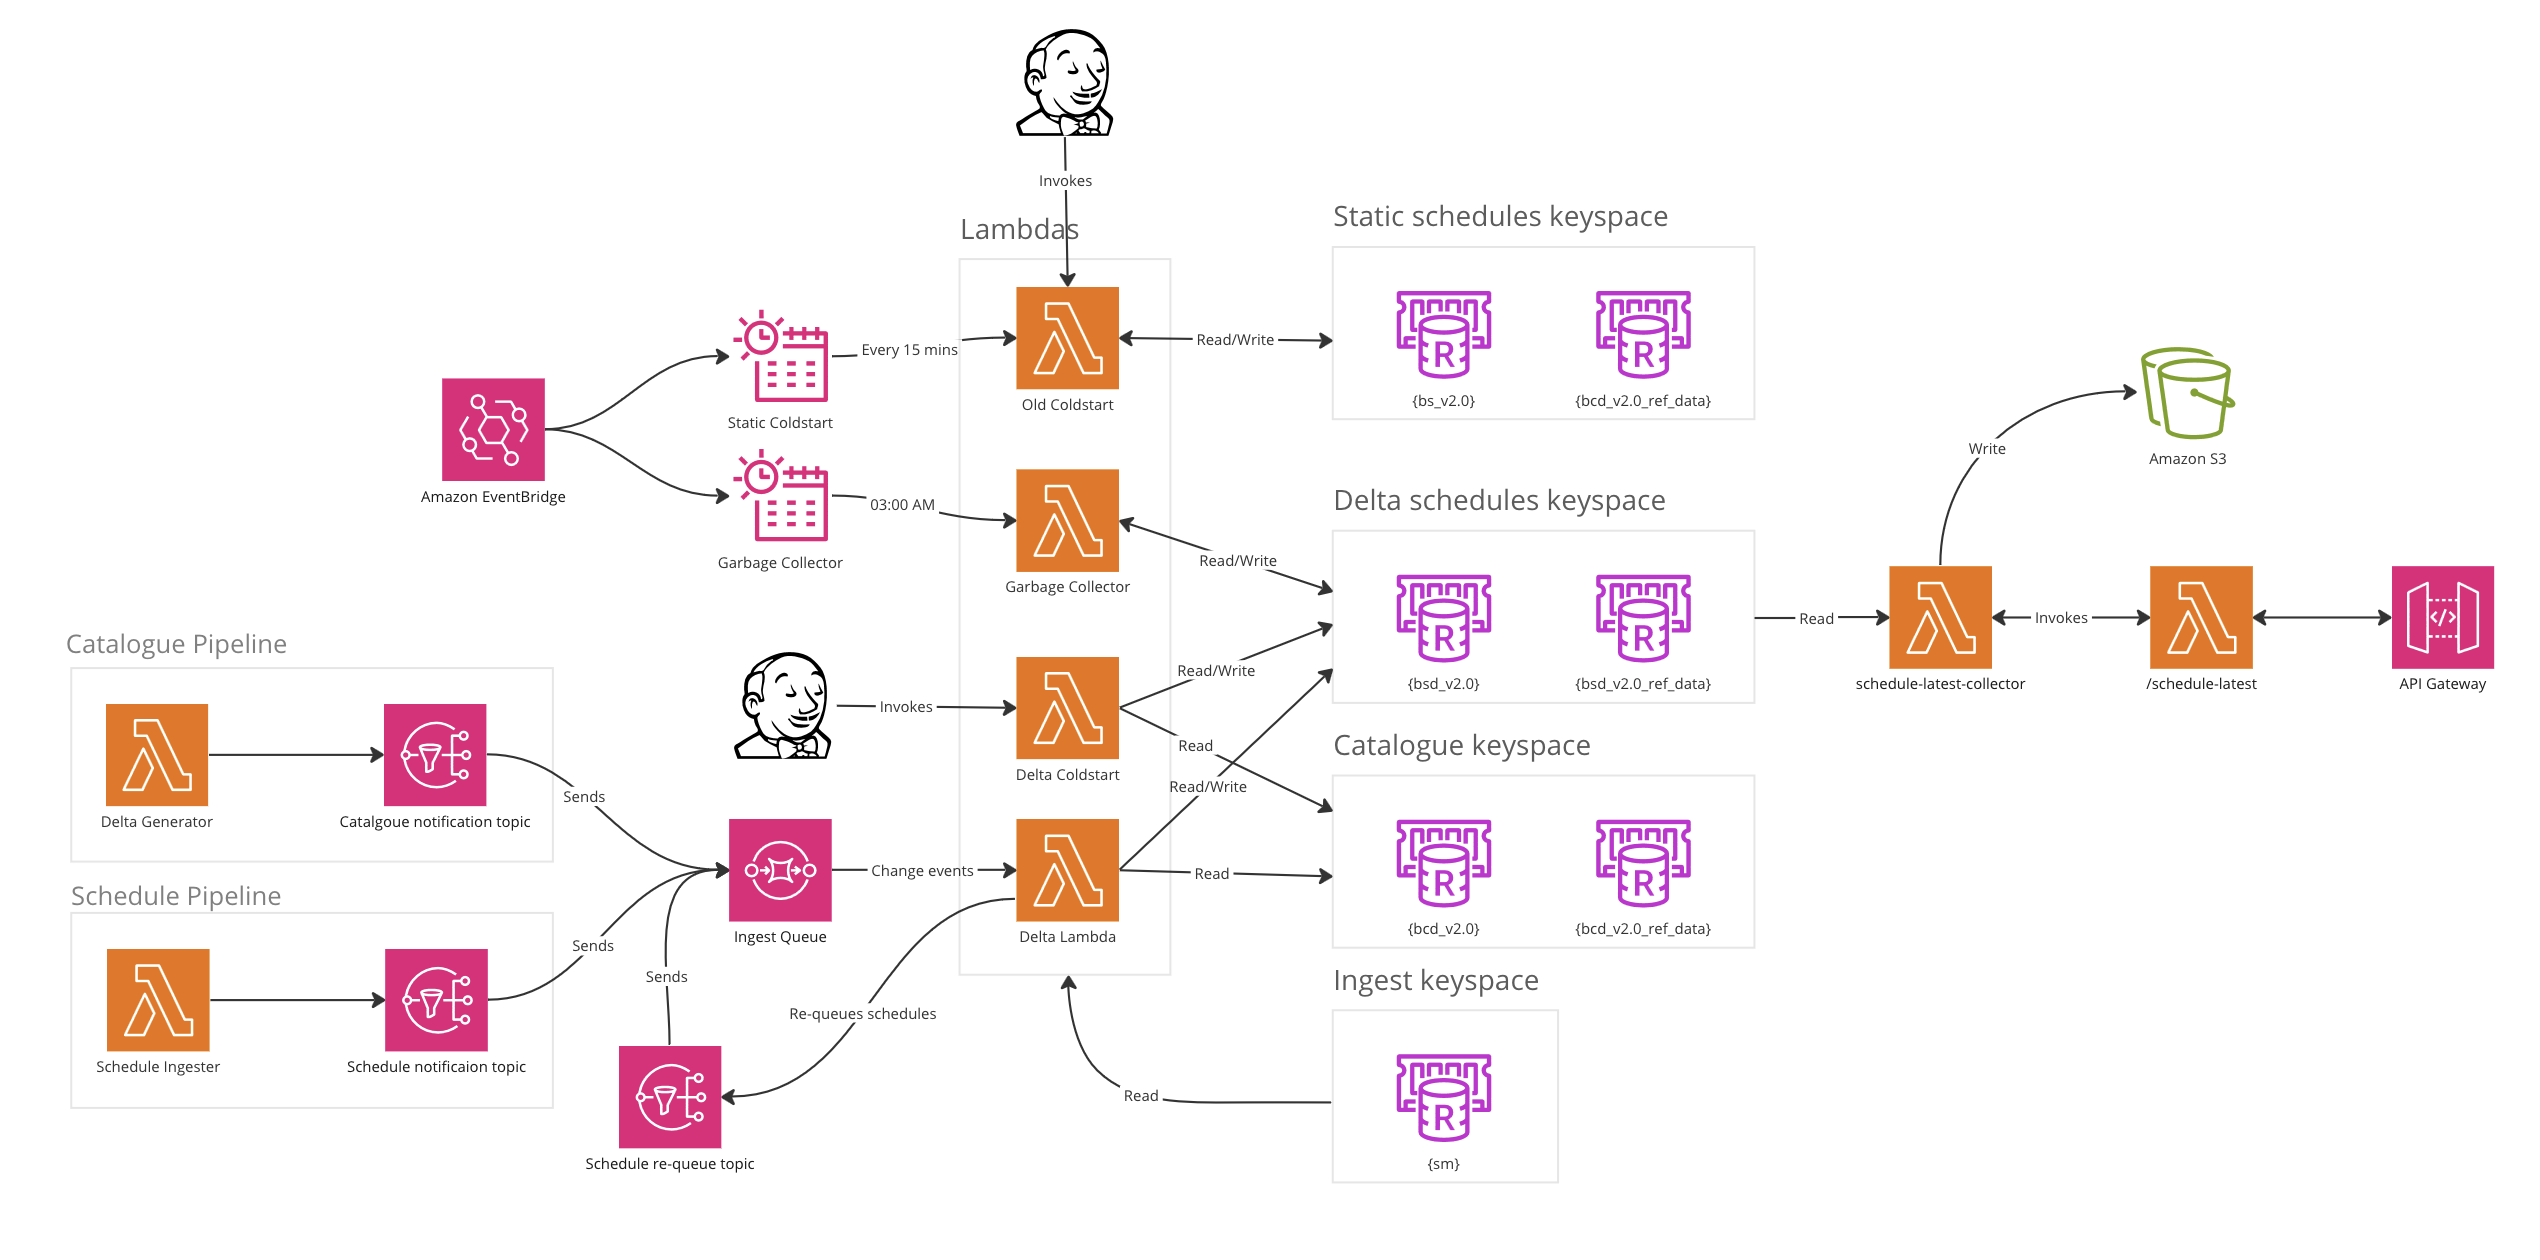
\includegraphics[width=20cm]{assets/outputs/finalArchitecture.png}
      \caption{Final architecture for project.}
      \label{fig:finalArchitecture}
    \end{figure}
  \end{landscape}

  \newpage
  \subsection{Dashboard}

  \textbf{Experience} - Dashboards have been created using a tool called Grafana (2024) that pulls metrics (Amazon Web Services, 2024m) from AWS and
  displays them all in one place. This allows us to check for anomalies and errors. Some metrics such as lambda run-times and invocations are provided by 
  AWS but custom metrics have also been created to track errors, redis writes and schedule re-queues. Metrics are collected during the run time of the 
  lambda using variations of the following code.

   \begin{lstlisting}[caption=Code used to update a metric\, this variation tracks a schedule delete.]
    monitoring.collect({
      typeId: 'Processing',
      result: 'throughput',
      dimensions: {
        ObjType: 'service_schedule',
        EventType: 'Delete'
      },
      value: 1
    })
  \end{lstlisting}

  \textbf{Reflection} - I've used metrics and dashboards throughout my time at the BBC so this is not something that is new to me. Usually the process of 
  adding these metrics is done at the very end of development. This stops monitoring during development which is only a negative. Due to the use of a spike 
  in this project we were able to know what metrics we wanted to track from the start and therefore added them along the way. This helped a lot as metrics on 
  both test and live could be compared to one another as a way to validate that changes had occurred.
  
  \vspace{0.2cm}
  \textbf{Action} - Continue to use spikes where necessary and put more thought into what kind of metrics we want to track before development starts.
  This allows comparisons between different dashboards as well as saves one or multiple extra tasks at the end of development to create the metrics and
  dashboards.

  \begin{figure}[H]
    \centering
    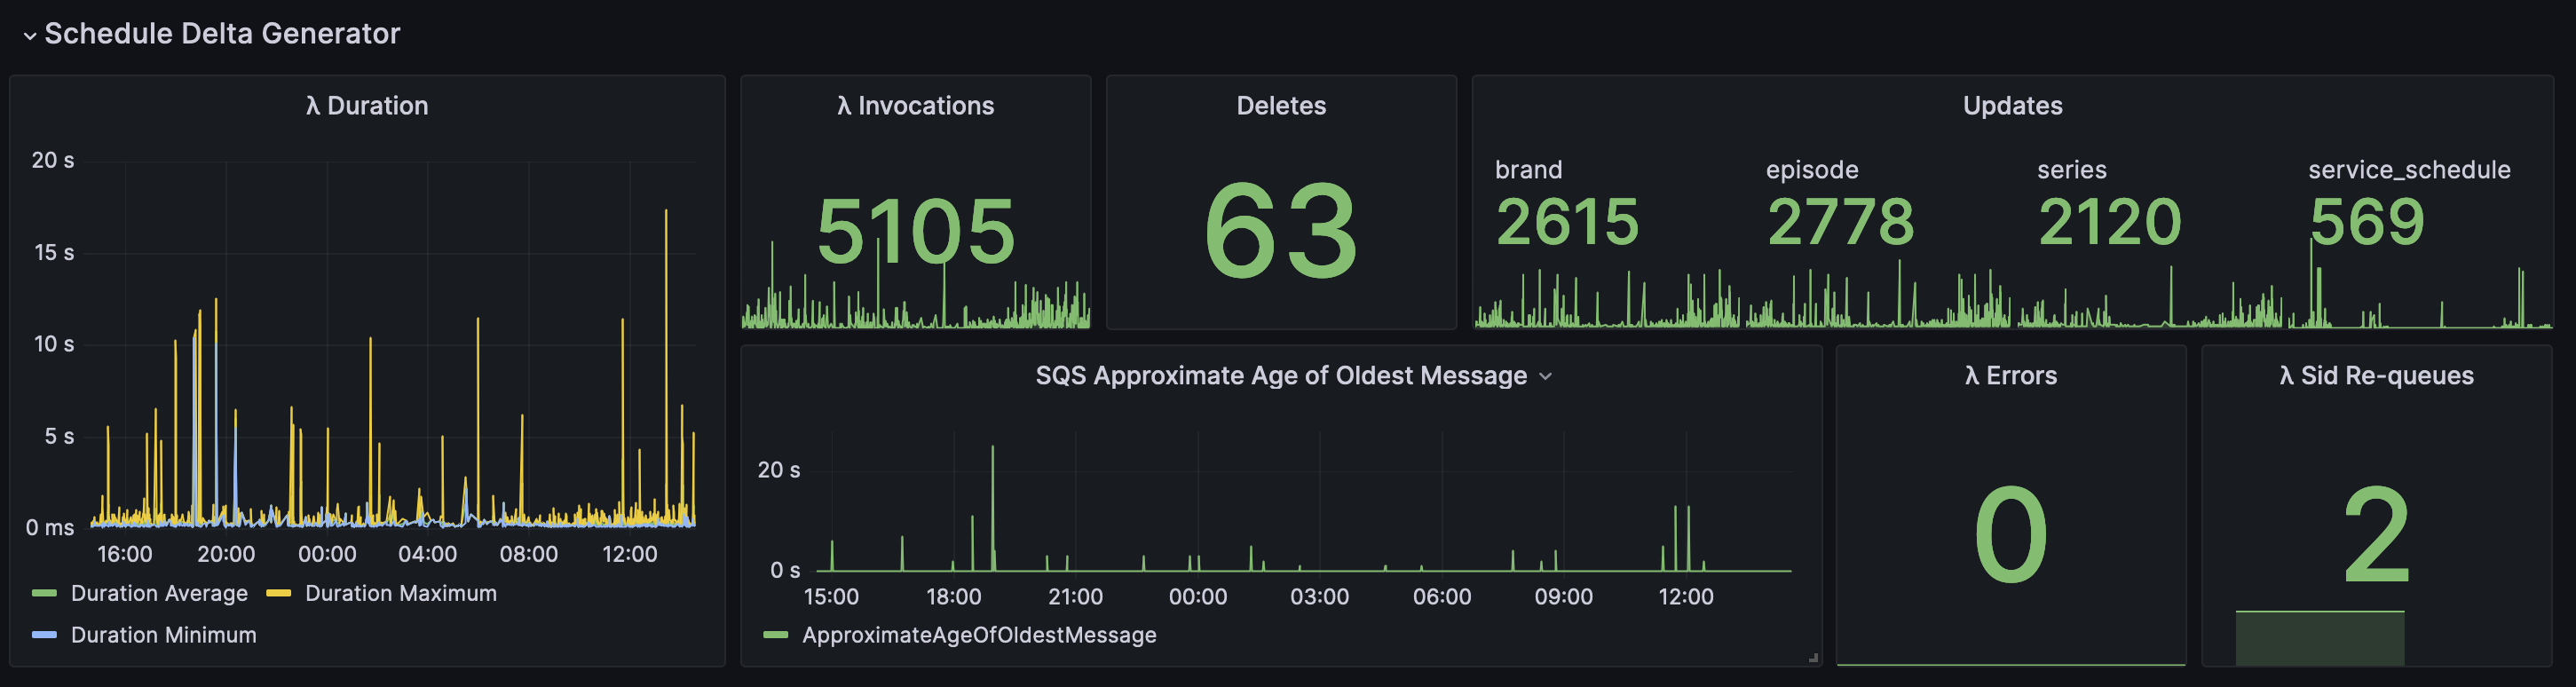
\includegraphics[width=12cm]{assets/outputs/dashboard.png}
    \caption{Created dashboard in Grafana.}
    \label{fig:dashboard}
  \end{figure}
  
  \newpage
  \subsection{Code Base and Commits}

  \textbf{Experience} - The project was created using JavaScript, alongside Cloudformation (Amazon Wrb Services, 2024n) for AWS resource provisioning and 
  Jenkins (2024) pipelines for CI/CD. This is our typical stack for all projects in our team. All unit tests were written using the Jest 
  (Meta Platforms, Inc, 2024) framework and were done alongside the development of tasks.

  \vspace{0.2cm}
  \textbf{Reflection} - Despite there being some questions over the architectural design, the team worked well to develop the final product, due to daily 
  discussion on how to tackle the problems that came up. It also helped that we stuck to known technologies and followed a similar working pattern to what 
  we usually do. In this aspect it could be argued that the right decision was made on architecture, as we could re-use a lot of code from elsewhere.
  However, as previously mentioned though it would be good to get more expertise and knowledge of newer/different solutions.

  There has been some talks through retrospectives (Atlassian, 2024) about using TypeScript (Microsoft, 2024) for our future projects. TypeScript has been 
  shown to lead to better code quality, less bugs and more understandable code (Merkel, 2021). In addition to this statically typed languages have been shown
  to help with bug fixes, especially around types (Okon and Hanenberg, 2016 and Kleinschmager et al, 2012).

  Once again the code works as expected and provides the correct output. New technologies and languages should be regarded as ways to improve in the future.
  Overall I'm happy with the work we did as a team, we ended up beating the estimated finish time by some way that was predicted by the burn-up charts and 
  I'm also happy that despite having to do a lot of other non-dev related tasks, I still managed to get a lot of work committed to the project.

  As a team we also tried to adhere to the Do not Repeat Yourself (DRY) principle throughout the project (Morais, 2023). This helps reduce number of lines of 
  code and  also stops the need to change code in multiple places due to slight changes in implementation detail. This could be seen in our decisions around the 
  coldstart in delta mode, as well as the shared API used to updated schedule items on catalogue update notifications.

  \vspace{0.2cm}
  \textbf{Action} - TypeScript would definitely help with code quality and other aspects in the future. However it is not worth re-writing everything at this
  stage and instead consider for new projects in the future. As previously mentioned continuous learning of new technologies is required to create the 
  best products possible, both from and external and internal perspective. 
  
  Continued retrospectives will help bring up some of these technologies and any other issue the team has.

  \begin{figure}[H]
    \centering
    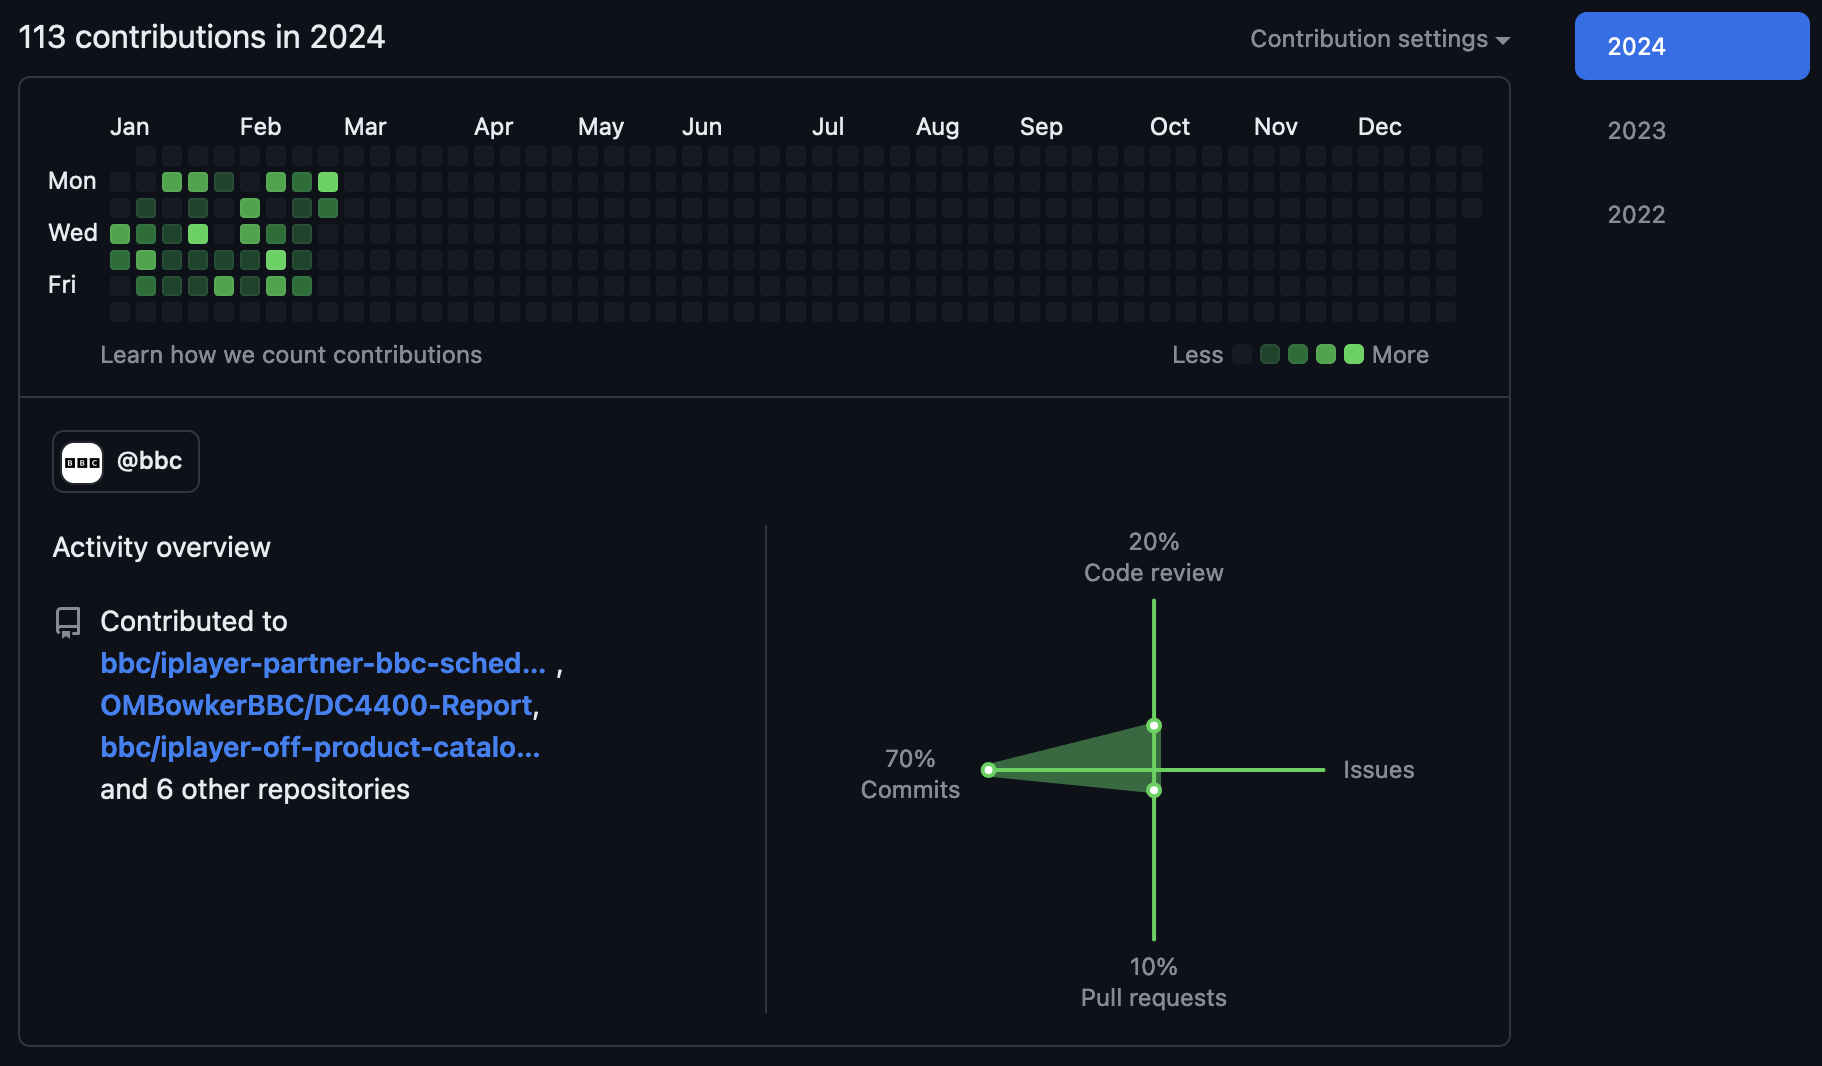
\includegraphics[width=6cm]{assets/outputs/githubContributions.png}
    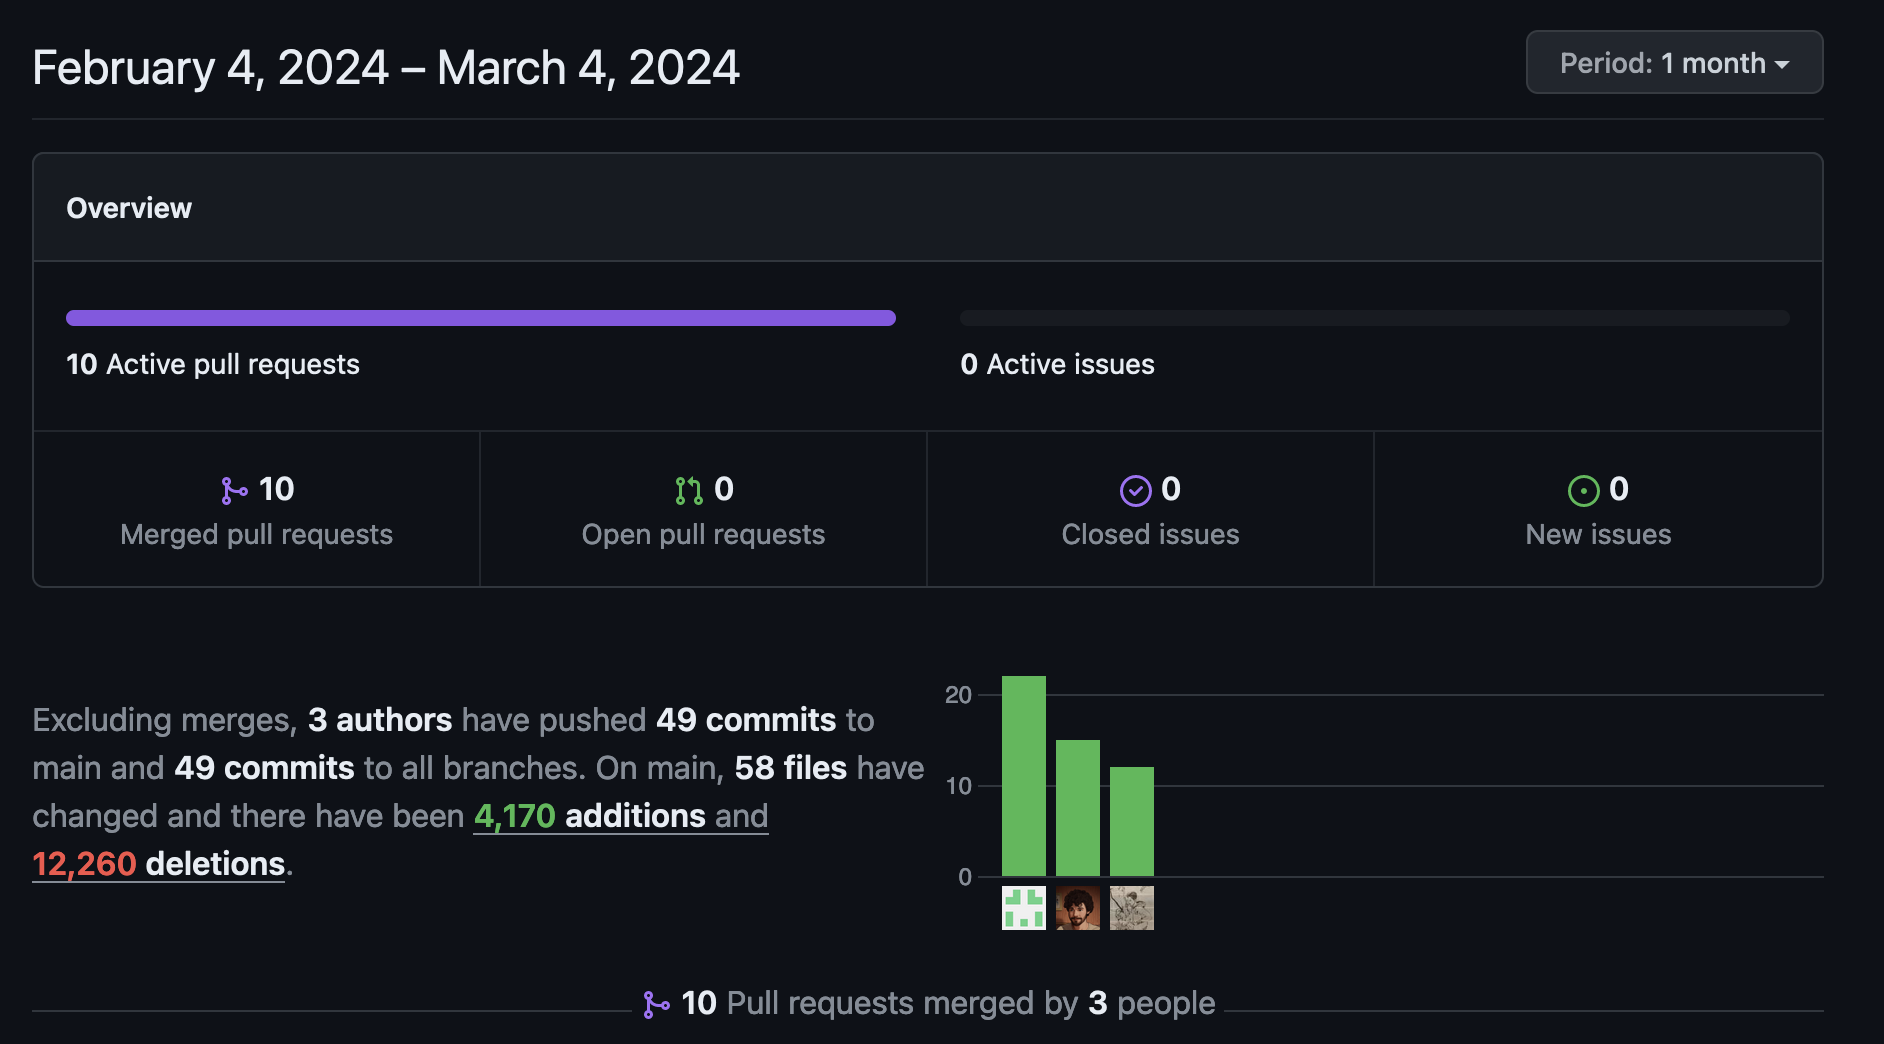
\includegraphics[width=6cm]{assets/outputs/scheduleGeneratorChanges.png}

    \caption{Github contributions for my work profile and the schedule generator project.}
    \label{fig:githubStats}
  \end{figure}

  \subsubsection{Visualtion of Changes}
  Due to the nature of the project, it's hard to see any visual output. Fot this reason I created a tool to show what notifications are coming 
  into the system. The code for this can be seen in \hyperref[sec:sec:AppendixG]{\textbf{Appendix G}}.

\newpage
